\documentclass{article}

\usepackage[utf8]{inputenc} 
\usepackage[russian]{babel} 
\usepackage{amsmath} 
\usepackage{hyperref} 
\usepackage{multicol}
\usepackage{graphicx}
\usepackage{amssymb}
\usepackage{tipa}
\graphicspath{{pictures/}}
\DeclareGraphicsExtensions{.pdf,.png,.jpg}

\title{Домашнее задание по АиСД №3}
\date{2020-06-07}
\author{Эмиль Гарипов M3138}
\usepackage[left=2cm,right=2cm,
top=2cm,bottom=2cm,bindingoffset=0cm]{geometry}

\begin{document}
\pagenumbering{gobble}
\newcommand{\RomanNumeralCaps}[1]
{\MakeUppercase{\romannumeral #1}}


\maketitle
\newpage
\pagenumbering{arabic}

\section*{Задача №1}
\subsection*{Предподсчет и описание структуры}	
\qquad
Для решения задачи рассмотрим, как меняются элементы массива $a$ после очередного запроса прибавления. Элемент $a_l$ увеличивается на $x$, элемент $a_{l + 1}$ увеличивается на $x + k$, элемент $a_{l + i}$ увеличивается на $x + (i - l) \cdot k$. Заведем массив $diff$, значение $diff_i$ будем вычислять как $diff_i = a_i - a_{i - 1}$, $diff_0$ положим равным $a_0$. Тогда при очередном запросе прибавления массив $diff$ меняется так, как показано на рисунке ниже (в кружок обведено то значение, на которое увеличается этот элемент массива): 
\begin{figure}[h]
	\center{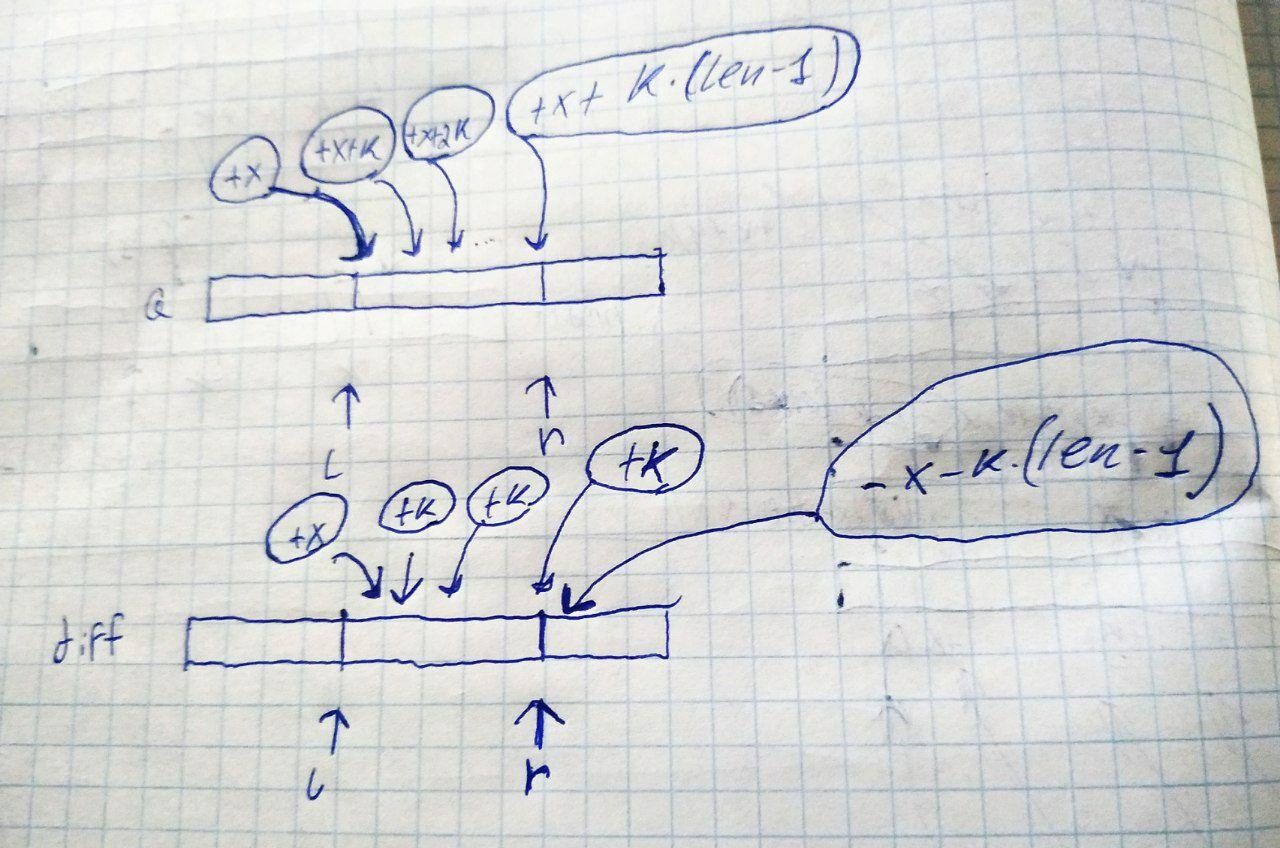
\includegraphics[scale=0.40]{hw3_1}}
	\caption{Изменение массива $diff$}
	\label{fig:diff}
\end{figure}

\qquad
Заметим, что для обработки запроса прибавления надо просто изменить массив $diff$ на отрезке \\ $[l; r + 1]$ соответстующим образом: прибавить на отрезке $[l + 1; r]$ значения $k$, прибавить значение $x$ в точке $l$ и прибавить значение $-x - k \cdot (len - 1)$ в точке $r + 1$ в массиве $diff$. Чтобы каждый запрос прибавления обрабатывать за $\mathcal{O}(1)$ будем вычислять значение $diff_i$ так: 
\begin{equation}
diff_i = \sum_{j = 0}^{i}prefdiff_j
\end{equation}

Для вычисления массива $diff$ сначала подсчиаем массив $prefdiff$, а далее, зная массив $diff$, посчитаем массив $a$, который и будет ответом на задачу. Осталось только понять как по запросам посчитать массив $prefdiff$. 

\qquad Рассмотрим изменения в массиве $prefdiff$ при одном запросе прибавления, эти изменения должны быть такими, чтобы при вычислении массива $diff$ по формуле $(1)$ он изменился так, как показано на Рис. 1. Так же заметим, что при прибавление в массиве $prefdiff$ в точке $i$ соответстует прибавлению всем элементам на суффиксе $[i; n]$ в массиве $prefdiff$. А значит для прибавления значения $x$ на каком-то отрезке $[l'; r']$ в массиве $diff$ нужно просто прибавить в точку $l'$ в массиве $prefdiff$ значение $x$, а в точке $(r' + 1)$ в массиве $prefdiff$ прибавить значение $-x$. 

\qquad Пользуясь этим фактом выполним все прибавления в массиве $diff$.  На Рис. 2 показано, какие именно значения куда надо прибавить (в прямоугольниках над индексом $i$ записаны те значения, которые необходимо прибавить в $i$-й элемент).

\subsection*{Решение и время работы} 
\qquad Итого, для решения необходимо выполнить описанные прибавления в массиве $prefdiff$ ($\mathcal{O}(m)$), затем по полученным сначениям посчитать массив $diff$ по формуле $(1)$ ($\mathcal{O}(n)$). И в конце посчитать массив $a$ по массиву $diff$ ($\mathcal{O}(n)$). Массив $a$ по понятным причинам вычисляется так: 
$$a_i = \sum_{j = 0}^{i}diff_i$$
\begin{figure}[h!]
	\center{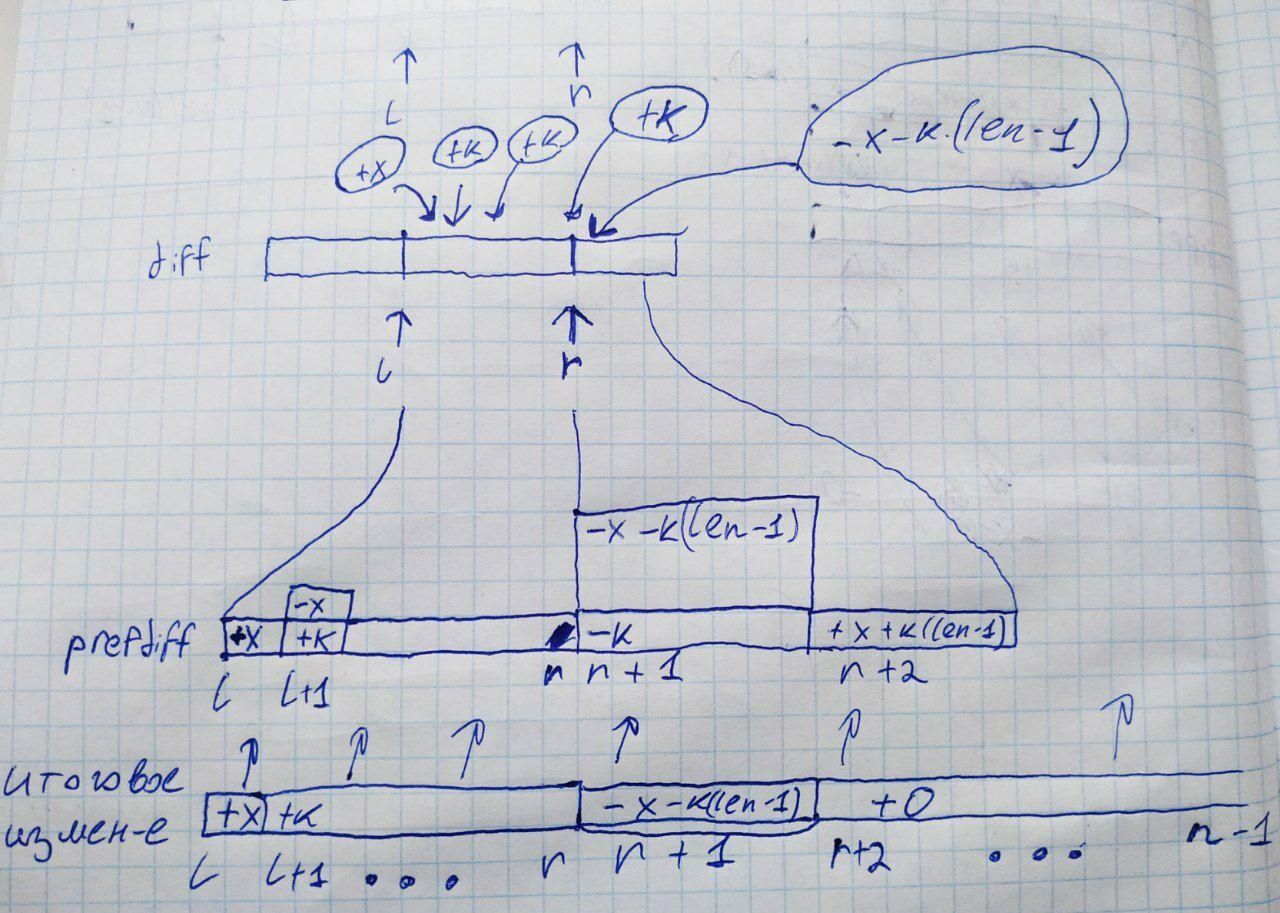
\includegraphics[scale=0.40]{hw3_2}}
	\caption{Сведение прибавления на отрезке к прибавлению в точке}
	\label{fig:image}
\end{figure}
Решение работает за $\mathcal{O}(n + m)$.


\section*{Задачи №4-5}
\subsection*{О Задачах 4-5}
Здесь описано решение Задачи №5, но оно включает в себя решение Задачи №4, так как Задача №4 являеется подзадачей Задачи №5.

\qquad
В решении используется нахождение $lca$ так называемыми <<Двоичными подъемами>>. Так же существует решение с поиском $lca$ при помощи данных heavy-light декомпозиции, что позволяет добиться времени предподсчета $\mathcal{O}(n)$. Но использование двоичных подъемов выбрано для краткости описания решения.
\subsection*{Предподсчет и описание структуры}
\qquad
По заданному дереву подсчитаем двоичные подъемы(для поиска LCA в дальшнейшем). Так же построим по дереву Heavy-Light декомпозицию, для каждого пути в heavy-light будем хранить два дерева отрезков, в одном (назовем его $t_1$) будем хранить самую ближайшую к корню непомеченную вершину, а во втором (назовем его $t_2$) самую далекую (глубокую) от корня непомеченную вершину. Стоит отметить, что вершины лежат в массиве, по которому строится дерево отрезков, в том порядке, в котором они находятся в пути в heavy-light декомпозиции(сверху-вниз). Для реализации этого дерево $t_1$ будет построено на минимум, в вершинах дерева отрезков будем хранить кортеж $<state; h; vertex>$, где  
\begin{equation*}
state = 
\begin{cases}
-1 &\text{, если вершина не помечена}\\
1 &\text{, если вершина помечена}
\end{cases}
\end{equation*} 
Тогда для поиска самой ближайшой к корню непомеченной вершины надо в дереве найти самый левый минимум. 

\qquad
Аналогичным образом (с точностью до замены минимума на максимум и изменении определения параметра $state$ в вершине дерева отрезков) можно реализовать дерево $t2$.
\subsection*{Ответы на запросы}
\ Для начала обозначим критерий того, что на пути из hld есть вершина, которая является ответом. Этим критерием мы будем пользоваться дальше. 

\qquad
\textbf{Критерий 1:} На пути есть вершина, которая является ответом, если самая ближайшая к корню непомеченная вершина на этом пути лежит выше текущей вершины (подробнее о том что такое текущая вершина написано ниже).

\qquad
\textbf{Док-во:} Предположим на пути больше нет непомеченных вершин, кроме самой ближайшей к корню на этом пути, тогда эта вершина является ответом. Если же есть еще непомеченные вершины, выше текущей, то самая дальная от корня (глубокая) и является ответом.

\quad 
Для проверки удовлетворения критерию будем использовать дерево отрезков $t1$, оно как раз хранит самую ближайшую к корню непомеченную вершину, причем эта вершина лежит в корне дерева отрезков, а значит мы будет узнавать эту вершину за $\mathcal{O}(1)$.
\begin{itemize}
	\item[\RomanNumeralCaps{1}]
	\subsubsection*{Запрос нахождения самого глубокого общего непомеченного предка} 
	
	\quad
	Имея подсчитанные двоичные подъемы найдем $lca(u, v)$, обозначим $lca(u, v) = t$. Очевидно, ответом являеется либо $t$, либо предки этой веришины $t$. Запустим алгоритм подъема по путям hld из $t$. Будем подниматься по путям из heavy-light декомпозиции дерева до тех пор, пока не дойдем до пути, удовлетворяющего \textbf{Критерию 1}. Причем подниматься будем так: из текущей вершины прыгнем в вершину, которая является началом пути в hld, а затем в ее предка, чтобы попасть на другой путь из hld. Когда дошли до пути, удовлетворяющего Критерию 1, найдем на этом пути самую дальную от корня (глубокую) вершину на отрезке от самой ближайшей к корню вершины этого пути до текущей. А это мы можем сделать при помощи нашего дерева отрезков $t2$ простым запросом самого правого максимума. 
	
	\qquad
	Итого ответ на запрос выполняется за $\mathcal{O}(\log_2(n))$, так как мы один раз обработаем запрос в дереве отрезков $t2$ за $\mathcal{O}(\log_2(n))$, сменим не более $\mathcal{O}(\log_2(n))$ путей и для каждого такого пути за $\mathcal{O}(1)$ будем проверять удовлетворение Критерию 1.
	\item[\RomanNumeralCaps{2}]
	\subsection*{Запрос снятия пометки с вершины}
	Для того чтобы снять пометку с вершины, просто изменим ее состояние в дереве отрезков на противоположное и обновим вершины дерева отрезков в $t1$ и $t2$ за $\mathcal{O}(\log_2(n))$.
	
	
\end{itemize}

\subsection*{Время работы}
Предподсчет выполняется за $\mathcal{O}(n\log_2{n})$, ответы на запросы за $\mathcal{O}(\log_2{n})$.


\end{document}
